\documentclass[border=18pt,tikz]{standalone}
\usepackage[T1]{fontenc}
\usepackage{helvet}
\renewcommand{\familydefault}{\sfdefault}
\usepackage{amsmath,amssymb}
\usepackage{xcolor}
\usepackage{tikz}
\usetikzlibrary{shapes.geometric, arrows.meta, positioning, calc, fit, backgrounds}

% ==============================================================================
% COLOR PALETTE (Publication-Quality IEEE Standards)
% ==============================================================================
\definecolor{primaryNavy}{HTML}{0A2540}      % Deep corporate/academic navy
\definecolor{secBlue}{HTML}{1E40AF}          % IEEE Royal blue
\definecolor{lightBlueBg}{HTML}{EFF6FF}      % Ice blue tint
\definecolor{darkBlue}{HTML}{0F172A}         % Slate midnight black
\definecolor{cardBorder}{HTML}{94A3B8}       % Slate border

% Offline Pipeline Palette (Cool Slate / Blue)
\definecolor{offlineBg}{HTML}{F8FAFC}        % Offline container background
\definecolor{offlineBorder}{HTML}{475569}    % Offline container border
\definecolor{datasetBlue}{HTML}{0284C7}      % Dataset accent
\definecolor{datasetBg}{HTML}{F0F9FF}        % Dataset card background
\definecolor{modelABg}{HTML}{EEF2FF}         % Model A box
\definecolor{modelBBg}{HTML}{F0FDF4}         % Model B box

% Online Runtime Palette (Teal / Emerald / Cyber)
\definecolor{onlineBg}{HTML}{F0FDFA}         % Online container background
\definecolor{onlineBorder}{HTML}{0D9488}     % Online container border
\definecolor{engineTeal}{HTML}{0F766E}       % Continuous Trust Engine
\definecolor{engineTealBg}{HTML}{CCFBF1}     % Engine background
\definecolor{scoreBlue}{HTML}{0369A1}        % Continuous Trust Score
\definecolor{scoreBlueBg}{HTML}{E0F2FE}      % Score background

% Decision Palette
\definecolor{acceptGreen}{HTML}{15803D}      % Accept branch
\definecolor{acceptBg}{HTML}{DCFCE7}         % Accept background
\definecolor{monitorAmber}{HTML}{B45309}     % Monitor branch
\definecolor{monitorBg}{HTML}{FEF3C7}        % Monitor background
\definecolor{isolateRed}{HTML}{B91C1C}       % Isolate branch
\definecolor{isolateBg}{HTML}{FEE2E2}        % Isolate background

% XAI Palette
\definecolor{xaiPurple}{HTML}{6B21A8}        % XAI accent
\definecolor{xaiPurpleBg}{HTML}{F3E8FF}      % XAI card background

% Backend & Database Palette
\definecolor{appBg}{HTML}{F8FAFC}            % App/Backend background
\definecolor{appBorder}{HTML}{334155}        % App/Backend border
\definecolor{fastapiGreen}{HTML}{059669}     % Backend accent
\definecolor{dbSlate}{HTML}{1E293B}          % Database header

% ==============================================================================
% TIKZ STYLE DEFINITIONS (Strictly Static & Overleaf-Compatible)
% ==============================================================================
\begin{document}
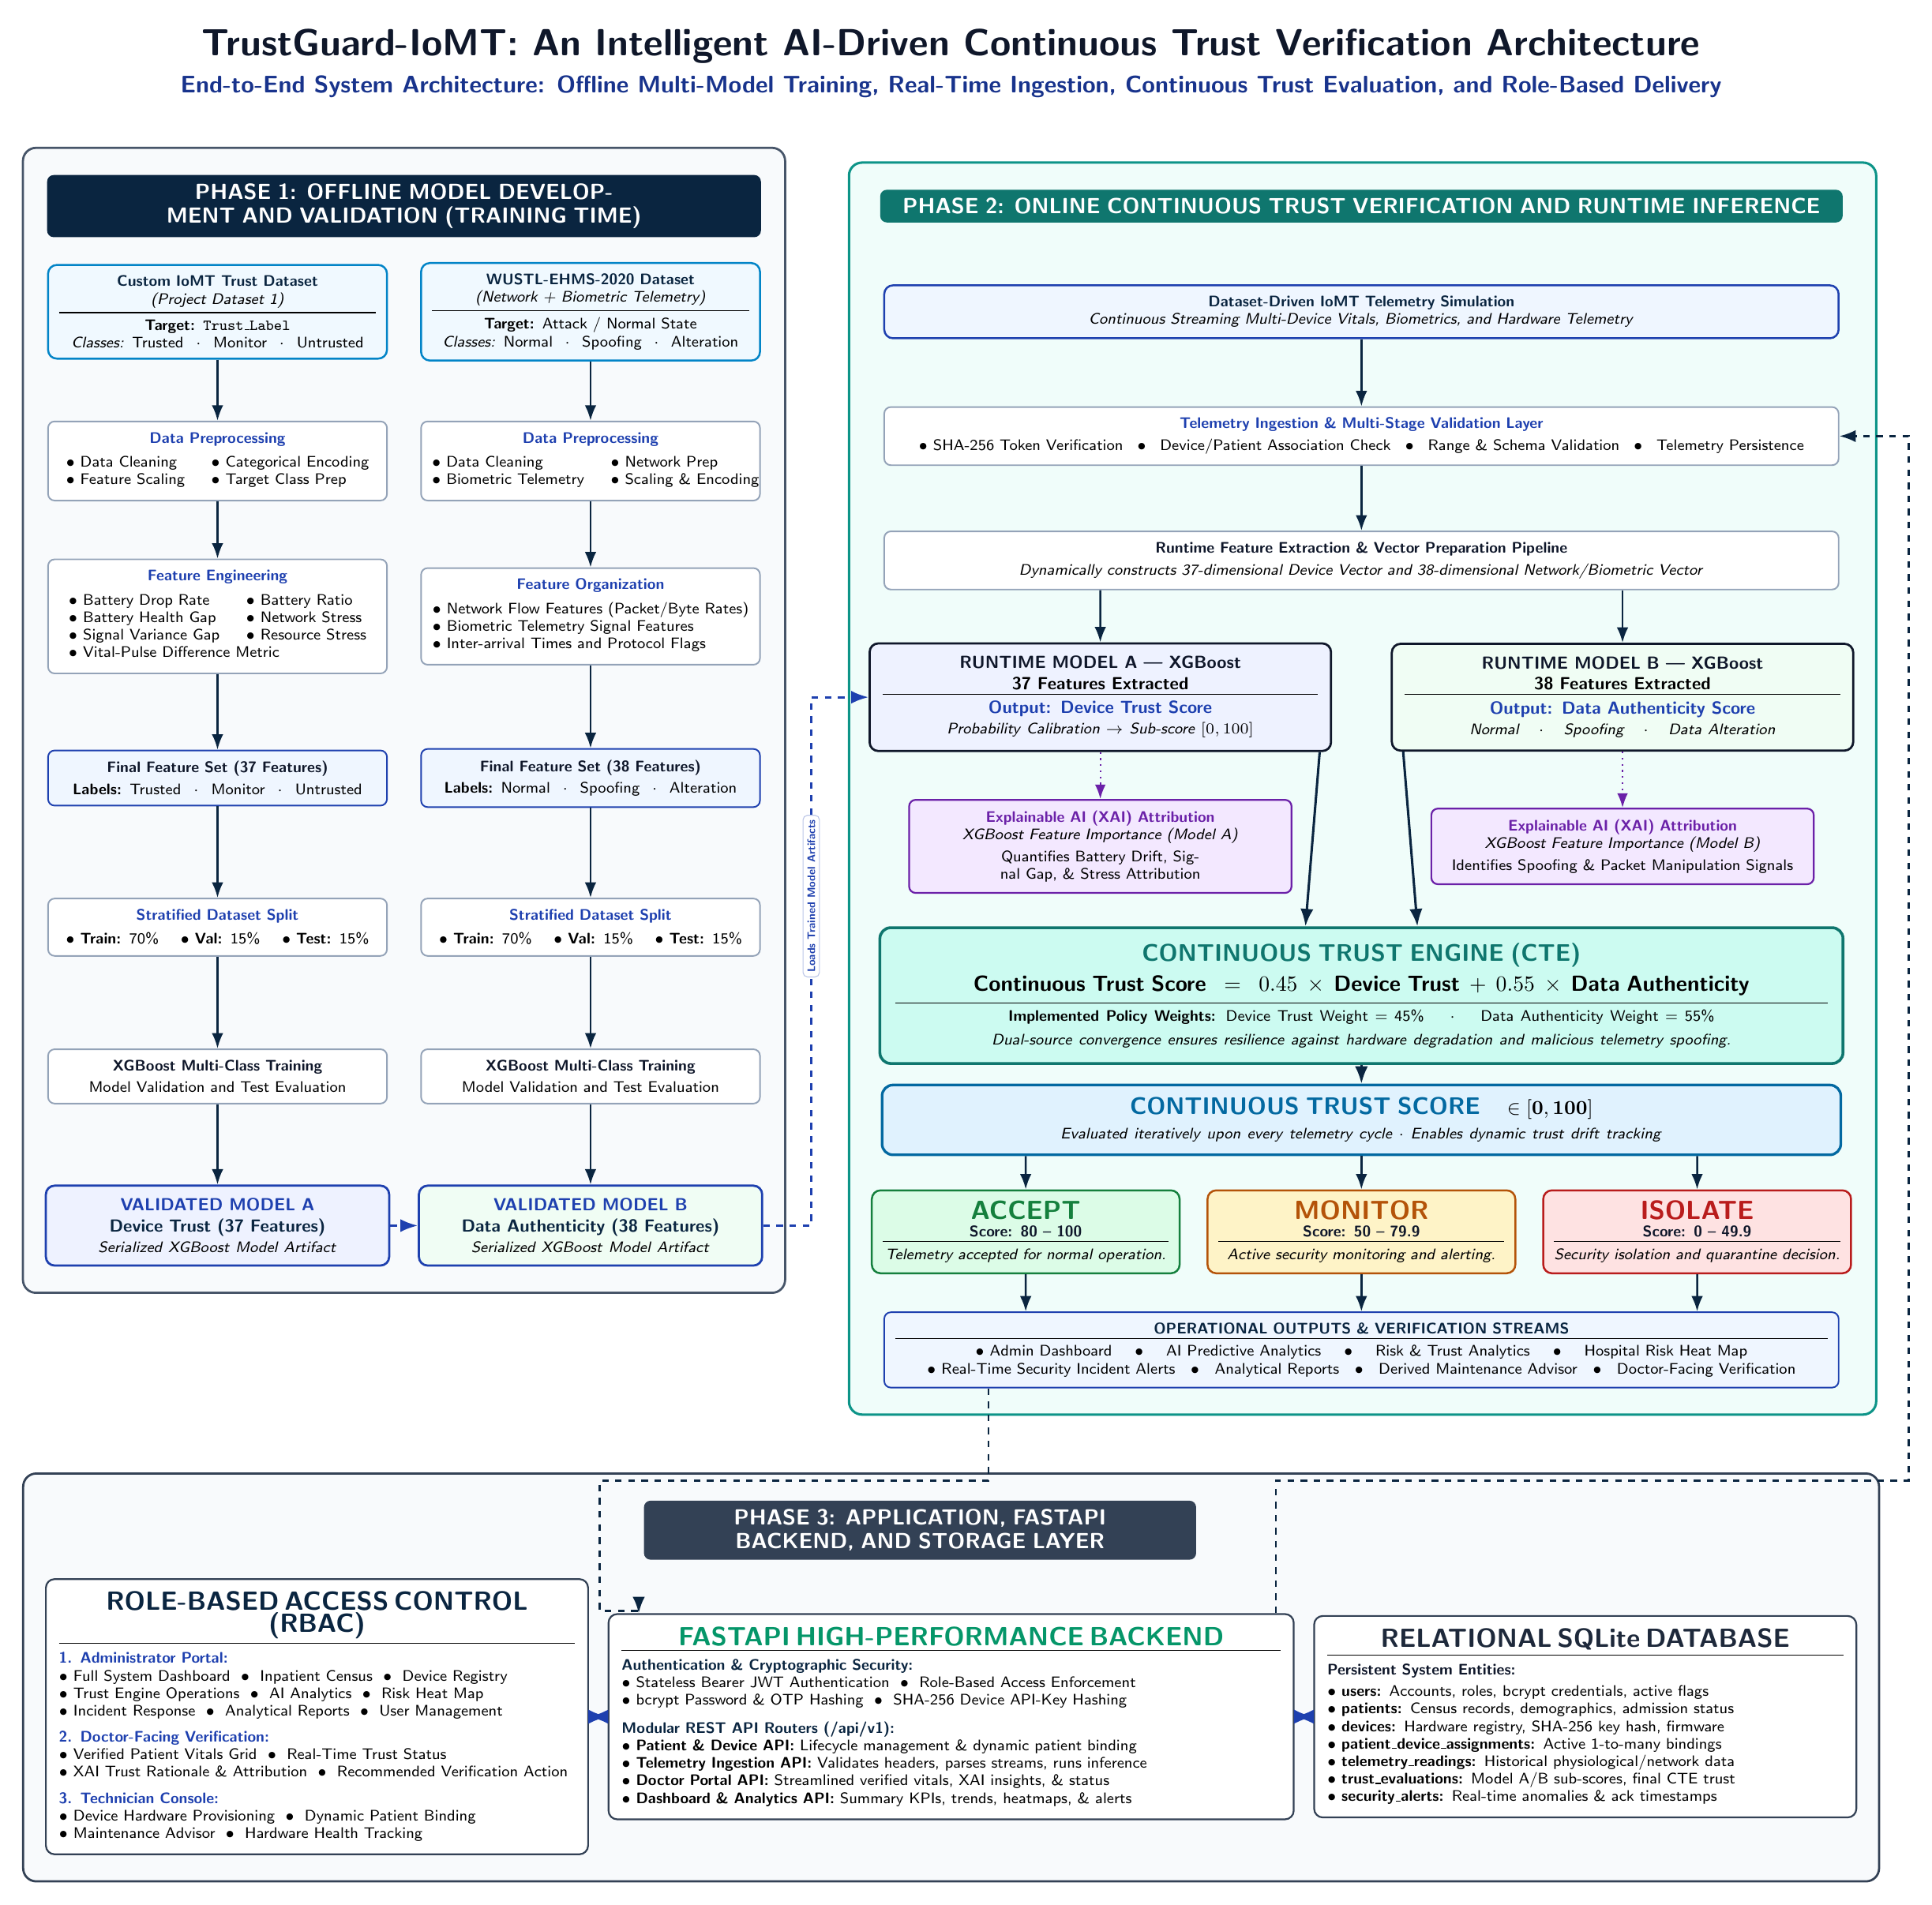
\begin{tikzpicture}[
  >=Latex,
  font=\small,
  % --- Process & Pipeline Nodes ---
  processNode/.style={
    rectangle, rounded corners=3pt, draw=cardBorder, line width=0.7pt,
    fill=white, align=center, inner sep=5pt, font=\scriptsize
  },
  datasetNode/.style={
    rectangle, rounded corners=4pt, draw=datasetBlue, line width=0.9pt,
    fill=datasetBg, align=center, inner sep=5pt, font=\scriptsize
  },
  splitNode/.style={
    rectangle, rounded corners=3pt, draw=secBlue, line width=0.7pt,
    fill=lightBlueBg, align=center, inner sep=5pt, font=\scriptsize
  },
  modelNode/.style={
    rectangle, rounded corners=4pt, draw=darkBlue, line width=1pt,
    fill=white, align=center, inner sep=6pt, font=\footnotesize
  },
  xaiNode/.style={
    rectangle, rounded corners=3pt, draw=xaiPurple, line width=0.8pt,
    fill=xaiPurpleBg, align=center, inner sep=5pt, font=\scriptsize
  },
  engineNode/.style={
    rectangle, rounded corners=5pt, draw=engineTeal, line width=1.3pt,
    fill=engineTealBg, align=center, inner sep=7pt
  },
  scoreNode/.style={
    rectangle, rounded corners=5pt, draw=scoreBlue, line width=1.2pt,
    fill=scoreBlueBg, align=center, inner sep=6pt
  },
  acceptNode/.style={
    rectangle, rounded corners=4pt, draw=acceptGreen, line width=0.9pt,
    fill=acceptBg, align=center, inner sep=5pt, font=\scriptsize
  },
  monitorNode/.style={
    rectangle, rounded corners=4pt, draw=monitorAmber, line width=0.9pt,
    fill=monitorBg, align=center, inner sep=5pt, font=\scriptsize
  },
  isolateNode/.style={
    rectangle, rounded corners=4pt, draw=isolateRed, line width=0.9pt,
    fill=isolateBg, align=center, inner sep=5pt, font=\scriptsize
  },
  systemLayerNode/.style={
    rectangle, rounded corners=4pt, draw=appBorder, line width=0.8pt,
    fill=white, align=left, inner sep=6pt, font=\scriptsize
  },
  headerBanner/.style={
    rectangle, rounded corners=3pt, line width=0.9pt,
    align=center, inner sep=4pt
  },
  % --- Connector Lines & Arrows ---
  dataArrow/.style={->, draw=primaryNavy, line width=0.9pt},
  offlineConn/.style={->, draw=secBlue, line width=1.1pt, dashed},
  xaiArrow/.style={->, draw=xaiPurple, line width=0.8pt, dotted},
  feedbackArrow/.style={->, draw=engineTeal, line width=0.9pt, dashed},
  layerArrow/.style={<->, draw=secBlue, line width=1.3pt},
]

% ==============================================================================
% TOP FIGURE TITLE & SUBTITLE (CLEANLY ELEVATED TO PREVENT ANY COLLISION)
% ==============================================================================
\node[align=center] (mainTitle) at (15.0, 3.4) {
  {\fontsize{18}{22}\selectfont\textbf{\color{darkBlue}TrustGuard-IoMT: An Intelligent AI-Driven Continuous Trust Verification Architecture}} \\[6pt]
  {\fontsize{10.5}{14}\selectfont\textbf{\color{secBlue!80!black}End-to-End System Architecture: Offline Multi-Model Training, Real-Time Ingestion, Continuous Trust Evaluation, and Role-Based Delivery}}
};

% ==============================================================================
% PHASE 1: OFFLINE MODEL DEVELOPMENT / TRAINING (LEFT COLUMN)
% Center: X = 6.2 | Width = 11.6cm | Header at Y = 1.1
% Model A Center: X = 3.2 (w=5.1cm) | Model B Center: X = 9.2 (w=5.1cm)
% ==============================================================================

% Centered Phase 1 Header Banner
\node[headerBanner, fill=primaryNavy, text=white, text width=11.2cm] (hdrPhase1) at (6.2, 1.1) {
  \textbf{\normalsize PHASE 1: OFFLINE MODEL DEVELOPMENT AND VALIDATION (TRAINING TIME)}
};

% --- MODEL A PIPELINE ---
\node[datasetNode, text width=5.1cm] (dsA) at (3.2, -0.6) {
  \textbf{\color{primaryNavy}Custom IoMT Trust Dataset} \\
  \textit{(Project Dataset 1)} \\
  \vspace{2pt}\hrule\vspace{3pt}
  \textbf{Target:} \texttt{Trust\_Label} \\
  \textit{Classes:} Trusted $\;\cdot\;$ Monitor $\;\cdot\;$ Untrusted
};

\node[processNode, text width=5.1cm] (prepA) at (3.2, -3.0) {
  \textbf{\color{secBlue}Data Preprocessing} \\
  \vspace{3pt}
  \begin{tabular}{@{}ll@{}}
  $\bullet$ Data Cleaning & $\bullet$ Categorical Encoding \\
  $\bullet$ Feature Scaling & $\bullet$ Target Class Prep
  \end{tabular}
};

\node[processNode, text width=5.1cm] (feA) at (3.2, -5.5) {
  \textbf{\color{secBlue}Feature Engineering} \\
  \vspace{3pt}
  \begin{tabular}{@{}ll@{}}
  $\bullet$ Battery Drop Rate & $\bullet$ Battery Ratio \\
  $\bullet$ Battery Health Gap & $\bullet$ Network Stress \\
  $\bullet$ Signal Variance Gap & $\bullet$ Resource Stress \\
  \multicolumn{2}{@{}l@{}}{$\bullet$ Vital-Pulse Difference Metric}
  \end{tabular}
};

\node[splitNode, text width=5.1cm] (featA) at (3.2, -8.1) {
  \textbf{\color{darkBlue}Final Feature Set (37 Features)} \\
  \vspace{2pt}
  \textbf{Labels:} Trusted $\;\cdot\;$ Monitor $\;\cdot\;$ Untrusted
};

\node[processNode, text width=5.1cm] (splitA) at (3.2, -10.5) {
  \textbf{\color{secBlue}Stratified Dataset Split} \\
  \vspace{3pt}
  $\bullet$ \textbf{Train:} 70\% $\quad\bullet$ \textbf{Val:} 15\% $\quad\bullet$ \textbf{Test:} 15\%
};

\node[processNode, text width=5.1cm] (trainA) at (3.2, -12.9) {
  \textbf{\color{darkBlue}XGBoost Multi-Class Training} \\
  \vspace{2pt}
  Model Validation and Test Evaluation
};

\node[modelNode, text width=5.1cm, draw=secBlue, fill=modelABg] (valModelA) at (3.2, -15.3) {
  \textbf{\color{secBlue}VALIDATED MODEL A} \\
  \textbf{\color{primaryNavy}Device Trust (37 Features)} \\
  \textit{\scriptsize Serialized XGBoost Model Artifact}
};

% Vertical Flow Model A
\draw[dataArrow] (dsA) -- (prepA);
\draw[dataArrow] (prepA) -- (feA);
\draw[dataArrow] (feA) -- (featA);
\draw[dataArrow] (featA) -- (splitA);
\draw[dataArrow] (splitA) -- (trainA);
\draw[dataArrow] (trainA) -- (valModelA);

% --- MODEL B PIPELINE ---
\node[datasetNode, text width=5.1cm] (dsB) at (9.2, -0.6) {
  \textbf{\color{primaryNavy}WUSTL-EHMS-2020 Dataset} \\
  \textit{(Network + Biometric Telemetry)} \\
  \vspace{2pt}\hrule\vspace{3pt}
  \textbf{Target:} Attack / Normal State \\
  \textit{Classes:} Normal $\;\cdot\;$ Spoofing $\;\cdot\;$ Alteration
};

\node[processNode, text width=5.1cm] (prepB) at (9.2, -3.0) {
  \textbf{\color{secBlue}Data Preprocessing} \\
  \vspace{3pt}
  \begin{tabular}{@{}ll@{}}
  $\bullet$ Data Cleaning & $\bullet$ Network Prep \\
  $\bullet$ Biometric Telemetry & $\bullet$ Scaling \& Encoding
  \end{tabular}
};

\node[processNode, text width=5.1cm] (feB) at (9.2, -5.5) {
  \textbf{\color{secBlue}Feature Organization} \\
  \vspace{3pt}
  \begin{tabular}{@{}l@{}}
  $\bullet$ Network Flow Features (Packet/Byte Rates) \\
  $\bullet$ Biometric Telemetry Signal Features \\
  $\bullet$ Inter-arrival Times and Protocol Flags
  \end{tabular}
};

\node[splitNode, text width=5.1cm] (featB) at (9.2, -8.1) {
  \textbf{\color{darkBlue}Final Feature Set (38 Features)} \\
  \vspace{2pt}
  \textbf{Labels:} Normal $\;\cdot\;$ Spoofing $\;\cdot\;$ Alteration
};

\node[processNode, text width=5.1cm] (splitB) at (9.2, -10.5) {
  \textbf{\color{secBlue}Stratified Dataset Split} \\
  \vspace{3pt}
  $\bullet$ \textbf{Train:} 70\% $\quad\bullet$ \textbf{Val:} 15\% $\quad\bullet$ \textbf{Test:} 15\%
};

\node[processNode, text width=5.1cm] (trainB) at (9.2, -12.9) {
  \textbf{\color{darkBlue}XGBoost Multi-Class Training} \\
  \vspace{2pt}
  Model Validation and Test Evaluation
};

\node[modelNode, text width=5.1cm, draw=secBlue, fill=modelBBg] (valModelB) at (9.2, -15.3) {
  \textbf{\color{secBlue}VALIDATED MODEL B} \\
  \textbf{\color{primaryNavy}Data Authenticity (38 Features)} \\
  \textit{\scriptsize Serialized XGBoost Model Artifact}
};

% Vertical Flow Model B
\draw[dataArrow] (dsB) -- (prepB);
\draw[dataArrow] (prepB) -- (feB);
\draw[dataArrow] (feB) -- (featB);
\draw[dataArrow] (featB) -- (splitB);
\draw[dataArrow] (splitB) -- (trainB);
\draw[dataArrow] (trainB) -- (valModelB);


% ==============================================================================
% PHASE 2: ONLINE CONTINUOUS TRUST VERIFICATION (RIGHT COLUMN)
% Center: X = 21.6 | Width = 15.6cm | Header at Y = 1.1
% ==============================================================================

% Centered Phase 2 Header Banner
\node[headerBanner, fill=engineTeal, text=white, text width=15.2cm] (hdrPhase2) at (21.6, 1.1) {
  \textbf{\normalsize PHASE 2: ONLINE CONTINUOUS TRUST VERIFICATION AND RUNTIME INFERENCE}
};

% Ingestion & Feature Prep
\node[datasetNode, fill=lightBlueBg, draw=secBlue, text width=15.0cm] (telemetrySim) at (21.6, -0.6) {
  \textbf{\color{primaryNavy}Dataset-Driven IoMT Telemetry Simulation} \\
  \textit{\scriptsize Continuous Streaming Multi-Device Vitals, Biometrics, and Hardware Telemetry}
};

\node[processNode, text width=15.0cm] (ingestBox) at (21.6, -2.6) {
  \textbf{\color{secBlue}Telemetry Ingestion \& Multi-Stage Validation Layer} \\
  \vspace{2pt}
  $\bullet$ SHA-256 Token Verification $\;\bullet\;$ Device/Patient Association Check $\;\bullet\;$ Range \& Schema Validation $\;\bullet\;$ Telemetry Persistence
};

\node[processNode, text width=15.0cm] (runtimePrep) at (21.6, -4.6) {
  \textbf{\color{darkBlue}Runtime Feature Extraction \& Vector Preparation Pipeline} \\
  \vspace{2pt}
  \textit{\scriptsize Dynamically constructs 37-dimensional Device Vector and 38-dimensional Network/Biometric Vector}
};

\draw[dataArrow] (telemetrySim) -- (ingestBox);
\draw[dataArrow] (ingestBox) -- (runtimePrep);

% Parallel Runtime Models (Model A: X = 17.4 | Model B: X = 25.8 | Width = 7.0cm)
\node[modelNode, text width=7.0cm, draw=darkBlue, fill=modelABg] (rtModelA) at (17.4, -6.8) {
  \textbf{\color{darkBlue}RUNTIME MODEL A — XGBoost} \\
  \textbf{37 Features Extracted} \\
  \vspace{2pt}\hrule\vspace{3pt}
  \textbf{\color{secBlue}Output: Device Trust Score} \\
  \textit{\scriptsize Probability Calibration $\rightarrow$ Sub-score $[0, 100]$}
};

\node[modelNode, text width=7.0cm, draw=darkBlue, fill=modelBBg] (rtModelB) at (25.8, -6.8) {
  \textbf{\color{darkBlue}RUNTIME MODEL B — XGBoost} \\
  \textbf{38 Features Extracted} \\
  \vspace{2pt}\hrule\vspace{3pt}
  \textbf{\color{secBlue}Output: Data Authenticity Score} \\
  \textit{\scriptsize Normal $\;\cdot\;$ Spoofing $\;\cdot\;$ Data Alteration}
};

% Parallel split from Runtime Prep
\draw[dataArrow] ($(runtimePrep.south) + (-4.2, 0)$) -- (rtModelA.north);
\draw[dataArrow] ($(runtimePrep.south) + (4.2, 0)$) -- (rtModelB.north);

% XAI Feature Importance Branches (Sized at 5.8cm width to guarantee open central corridor)
\node[xaiNode, text width=5.8cm] (xaiA) at (17.4, -9.2) {
  \textbf{\color{xaiPurple}Explainable AI (XAI) Attribution} \\
  \textit{XGBoost Feature Importance (Model A)} \\
  \vspace{2pt}
  \scriptsize Quantifies Battery Drift, Signal Gap, \& Stress Attribution
};

\node[xaiNode, text width=5.8cm] (xaiB) at (25.8, -9.2) {
  \textbf{\color{xaiPurple}Explainable AI (XAI) Attribution} \\
  \textit{XGBoost Feature Importance (Model B)} \\
  \vspace{2pt}
  \scriptsize Identifies Spoofing \& Packet Manipulation Signals
};

% Dotted XAI Explanation arrows from Models to XAI
\draw[xaiArrow] (rtModelA.south) -- (xaiA.north);
\draw[xaiArrow] (rtModelB.south) -- (xaiB.north);

% --- OFFLINE-TO-ONLINE MODEL LOADING CONNECTORS ---
% Distinct gap between Validated Model A and Model B, routing cleanly through channel center X = 12.75.
\draw[offlineConn] (valModelA.east) -- (valModelB.west);
\draw[offlineConn] (valModelB.east) -- (12.75, -15.3) -- (12.75, -6.8) -- (rtModelA.west);
\node[font=\tiny\bfseries, text=secBlue, fill=white, draw=secBlue!30, rounded corners=2pt, inner sep=2pt, rotate=90] at (12.75, -10.0) {Loads Trained Model Artifacts};

% --- CONTINUOUS TRUST ENGINE ---
\node[engineNode, text width=15.0cm] (trustEngine) at (21.6, -11.6) {
  \textbf{\fontsize{11}{13}\selectfont\color{engineTeal}CONTINUOUS TRUST ENGINE (CTE)} \\
  \vspace{3pt}
  {\fontsize{10}{12}\selectfont\textbf{$\text{Continuous Trust Score} = 0.45 \times \text{Device Trust} + 0.55 \times \text{Data Authenticity}$}} \\
  \vspace{3pt}\hrule\vspace{3pt}
  \scriptsize\textbf{Implemented Policy Weights:} Device Trust Weight = 45\% $\;\cdot\;$ Data Authenticity Weight = 55\% \\
  \textit{\scriptsize Dual-source convergence ensures resilience against hardware degradation and malicious telemetry spoofing.}
};

% Direct converging outputs from Models into CTE (100% straight vertical arrows landing directly on top border of CTE)
\draw[dataArrow, line width=1.1pt] ($(rtModelA.south east) + (-0.2, 0)$) -- ($(trustEngine.north) + (-0.9, 0)$);
\draw[dataArrow, line width=1.1pt] ($(rtModelB.south west) + (0.2, 0)$) -- ($(trustEngine.north) + (0.9, 0)$);

% --- CONTINUOUS TRUST SCORE ---
\node[scoreNode, text width=15.0cm] (trustScore) at (21.6, -13.6) {
  \textbf{\fontsize{10.5}{12.5}\selectfont\color{scoreBlue}CONTINUOUS TRUST SCORE} $\quad\mathbf{\in [0, 100]}$ \\
  \textit{\scriptsize Evaluated iteratively upon every telemetry cycle $\cdot$ Enables dynamic trust drift tracking}
};

\draw[dataArrow, line width=1.1pt] (trustEngine) -- (trustScore);

% --- TRUST DECISION BOUNDARIES ---
\node[acceptNode, text width=4.6cm] (decAccept) at (16.2, -15.4) {
  \textbf{\color{acceptGreen}\large ACCEPT} \\
  \textbf{\color{darkBlue}Score: 80 -- 100} \\
  \vspace{2pt}\hrule\vspace{3pt}
  \textit{\scriptsize Telemetry accepted for normal operation.}
};

\node[monitorNode, text width=4.6cm] (decMonitor) at (21.6, -15.4) {
  \textbf{\color{monitorAmber}\large MONITOR} \\
  \textbf{\color{darkBlue}Score: 50 -- 79.9} \\
  \vspace{2pt}\hrule\vspace{3pt}
  \textit{\scriptsize Active security monitoring and alerting.}
};

\node[isolateNode, text width=4.6cm] (decIsolate) at (27.0, -15.4) {
  \textbf{\color{isolateRed}\large ISOLATE} \\
  \textbf{\color{darkBlue}Score: 0 -- 49.9} \\
  \vspace{2pt}\hrule\vspace{3pt}
  \textit{\scriptsize Security isolation and quarantine decision.}
};

% Downward flow from Score to 3 Decision Branches
\draw[dataArrow] ($(trustScore.south) + (-5.4, 0)$) -- (decAccept.north);
\draw[dataArrow] (trustScore.south) -- (decMonitor.north);
\draw[dataArrow] ($(trustScore.south) + (5.4, 0)$) -- (decIsolate.north);

% --- OPERATIONAL OUTPUTS ---
\node[processNode, fill=lightBlueBg, draw=secBlue, text width=15.0cm] (opsOutputs) at (21.6, -17.3) {
  \textbf{\color{primaryNavy}OPERATIONAL OUTPUTS \& VERIFICATION STREAMS} \\
  \vspace{2pt}\hrule\vspace{3pt}
  $\bullet$ Admin Dashboard $\;\bullet\;$ AI Predictive Analytics $\;\bullet\;$ Risk \& Trust Analytics $\;\bullet\;$ Hospital Risk Heat Map \\
  $\bullet$ Real-Time Security Incident Alerts $\;\bullet\;$ Analytical Reports $\;\bullet\;$ Derived Maintenance Advisor $\;\bullet\;$ Doctor-Facing Verification
};

\draw[dataArrow] (decAccept.south) -- ($(opsOutputs.north) + (-5.4, 0)$);
\draw[dataArrow] (decMonitor.south) -- (opsOutputs.north);
\draw[dataArrow] (decIsolate.south) -- ($(opsOutputs.north) + (5.4, 0)$);


% ==============================================================================
% PHASE 3: APPLICATION, FASTAPI BACKEND, AND STORAGE LAYER (BOTTOM TIER)
% Shifted down with clear 1.2cm vertical gap separating from Phase 2 container!
% Center: X = 15.0 | Total Width = 29.2cm | Header at Y = -20.2
% User: X = 4.8 (w=8.4cm) | Backend: X = 15.0 (w=10.6cm) | DB: X = 25.2 (w=8.4cm)
% ==============================================================================

% Centered Phase 3 Header Banner (Positioned at X = 14.5 with width 8.6cm, giving >1.2cm open clearance on both sides)
\node[headerBanner, fill=appBorder, text=white, text width=8.6cm] (hdrPhase3) at (14.5, -20.2) {
  \textbf{\normalsize PHASE 3: APPLICATION, FASTAPI BACKEND, AND STORAGE LAYER}
};

% User / RBAC Layer
\node[systemLayerNode, text width=8.3cm] (userLayer) at (4.8, -23.2) {
  \centering\textbf{\color{primaryNavy}\large ROLE-BASED ACCESS CONTROL (RBAC)} \\
  \vspace{2pt}\hrule\vspace{4pt}
  \raggedright
  \textbf{\color{secBlue}1. Administrator Portal:} \\
  $\bullet$ Full System Dashboard $\;\bullet\;$ Inpatient Census $\;\bullet\;$ Device Registry \\
  $\bullet$ Trust Engine Operations $\;\bullet\;$ AI Analytics $\;\bullet\;$ Risk Heat Map \\
  $\bullet$ Incident Response $\;\bullet\;$ Analytical Reports $\;\bullet\;$ User Management \\[4pt]
  \textbf{\color{secBlue}2. Doctor-Facing Verification:} \\
  $\bullet$ Verified Patient Vitals Grid $\;\bullet\;$ Real-Time Trust Status \\
  $\bullet$ XAI Trust Rationale \& Attribution $\;\bullet\;$ Recommended Verification Action \\[4pt]
  \textbf{\color{secBlue}3. Technician Console:} \\
  $\bullet$ Device Hardware Provisioning $\;\bullet\;$ Dynamic Patient Binding \\
  $\bullet$ Maintenance Advisor $\;\bullet\;$ Hardware Health Tracking
};

% FastAPI Backend Layer
\node[systemLayerNode, text width=10.6cm] (backendLayer) at (15.0, -23.2) {
  \centering\textbf{\color{fastapiGreen}\large FASTAPI HIGH-PERFORMANCE BACKEND} \\
  \vspace{2pt}\hrule\vspace{4pt}
  \raggedright
  \textbf{\color{primaryNavy}Authentication \& Cryptographic Security:} \\
  $\bullet$ Stateless Bearer JWT Authentication $\;\bullet\;$ Role-Based Access Enforcement \\
  $\bullet$ bcrypt Password \& OTP Hashing $\;\bullet\;$ SHA-256 Device API-Key Hashing \\[5pt]
  \textbf{\color{primaryNavy}Modular REST API Routers (/api/v1):} \\
  $\bullet$ \textbf{Patient \& Device API:} Lifecycle management \& dynamic patient binding \\
  $\bullet$ \textbf{Telemetry Ingestion API:} Validates headers, parses streams, runs inference \\
  $\bullet$ \textbf{Doctor Portal API:} Streamlined verified vitals, XAI insights, \& status \\
  $\bullet$ \textbf{Dashboard \& Analytics API:} Summary KPIs, trends, heatmaps, \& alerts
};

% SQLite Database Layer
\node[systemLayerNode, text width=8.3cm] (dbLayer) at (25.2, -23.2) {
  \centering\textbf{\color{dbSlate}\large RELATIONAL SQLite DATABASE} \\
  \vspace{2pt}\hrule\vspace{4pt}
  \raggedright
  \textbf{\color{darkBlue}Persistent System Entities:} \\
  \vspace{2pt}
  $\bullet$ \textbf{users:} Accounts, roles, bcrypt credentials, active flags \\
  $\bullet$ \textbf{patients:} Census records, demographics, admission status \\
  $\bullet$ \textbf{devices:} Hardware registry, SHA-256 key hash, firmware \\
  $\bullet$ \textbf{patient\_device\_assignments:} Active 1-to-many bindings \\
  $\bullet$ \textbf{telemetry\_readings:} Historical physiological/network data \\
  $\bullet$ \textbf{trust\_evaluations:} Model A/B sub-scores, final CTE trust \\
  $\bullet$ \textbf{security\_alerts:} Real-time anomalies \& ack timestamps
};

% Clean Horizontal bidirectional connections in System Layer
\draw[layerArrow] (userLayer.east) -- (backendLayer.west);
\draw[layerArrow] (backendLayer.east) -- (dbLayer.west);

% Vertical integration connectors between tiers:
% 1. Operational Outputs to FastAPI Backend (Strictly orthogonal path routing around the left of Phase 3 header, landing precisely on backendLayer border)
\draw[dataArrow, dashed, line width=1.0pt] ($(opsOutputs.south) + (-6.0, 0)$) |- (9.35, -19.4) -- (9.35, -21.5) -| ($(backendLayer.north west) + (0.5, 0)$);

% 2. FastAPI Backend to Ingestion Layer (Strictly orthogonal path routing around the right of Phase 3 header with wide margin at X = 30.4, never touching borders)
\draw[dataArrow, dashed, line width=1.0pt] ($(backendLayer.north east) + (-0.3, 0)$) |- (30.4, -19.4) -- (30.4, -2.6) -- (ingestBox.east);


% ==============================================================================
% BACKGROUND CONTAINERS (CLEAN, UNCLUTTERED, COMPLETELY SEPARATED)
% ==============================================================================
\begin{scope}[on background layer]
  % Container 1: Offline Model Training
  \node[
    rectangle, rounded corners=6pt, draw=offlineBorder, line width=1pt,
    fill=offlineBg, fit={(hdrPhase1) (dsA) (valModelA) (dsB) (valModelB)},
    inner xsep=10pt, inner ysep=12pt
  ] (offlineBox) {};

  % Container 2: Online Continuous Trust Verification
  \node[
    rectangle, rounded corners=6pt, draw=onlineBorder, line width=1.1pt,
    fill=onlineBg, fit={(hdrPhase2) (telemetrySim) (rtModelB) (trustEngine) (trustScore) (decAccept) (decIsolate) (opsOutputs)},
    inner xsep=10pt, inner ysep=12pt
  ] (onlineBox) {};

  % Container 3: Application, Backend & Database Layer (Cleanly separated from Phase 2 container with visible open space)
  \node[
    rectangle, rounded corners=6pt, draw=appBorder, line width=1pt,
    fill=appBg, fit={(hdrPhase3) (userLayer) (backendLayer) (dbLayer)},
    inner xsep=10pt, inner ysep=12pt
  ] (sysBox) {};
\end{scope}

\end{tikzpicture}
\end{document}
